{\bfseries Grover con búsqueda de una solución.

Definimos los estados
$$
    \ket{G} = \frac{1}{\sqrt{M}} \sum_{x \in \text{soluciones}} \ket{x}, \qquad \ket{B} = \frac{1}{\sqrt{N-M}} \sum_{x \notin \text{soluciones}} \ket{x}.
$$

El estado inicial es
$$
    \ket{\psi} = H^{\otimes n} \ket{0}^{\otimes n} = \sqrt{\frac{M}{N}}\ket{G} + \sqrt{\frac{N-M}{N}}\ket{B} = \sin\theta\,\ket{G} + \cos\theta\,\ket{B},
$$
con $\sin\theta = \sqrt{M/N}$.

El oráculo de fase $U_f$ cambia el signo de los estados solución:
$$
    U_f \ket{G} = -\ket{G}, \qquad U_f \ket{B} = \ket{B}.
$$

En el plano $\{\ket{G}, \ket{B}\}$, $U_f$ es una reflexión sobre el eje perpendicular a $\ket{G}$. El operador de difusión $U_{\psi^\perp} = 2\ket{\psi}\bra{\psi} - I$ es la reflexión sobre el eje $\ket{\psi}$. El producto $G = U_{\psi^\perp} U_f$ es entonces una rotación de ángulo $2\theta$ en ese plano (no confundir al operador $G$ con el estado ``bueno'', $\ket{G}$).

Aplicando esta rotación al estado inicial obtenemos
$$
    G\ket{\psi} = \sin(3\theta)\,\ket{G} + \cos(3\theta)\,\ket{B}.
$$
}

\begin{figure}[H]
    \begin{center}
        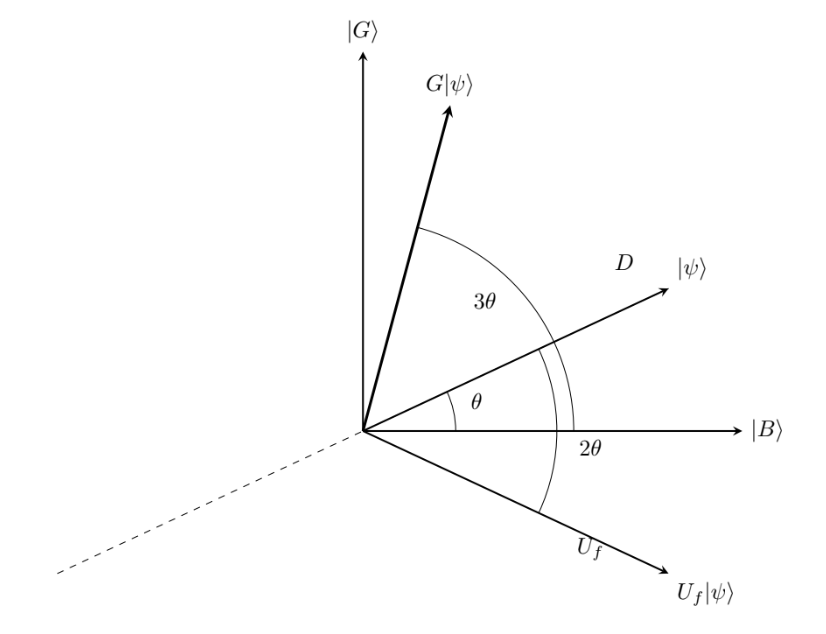
\includegraphics[width=10cm]{resources/img2.png}
    \end{center}
\end{figure}

{\bfseries Ejercicio: Sea una base de datos de tamaño $N=16$ (es decir, $n=4$ qubits). Suponga que hay una única solución ($M=1$), marcada por la función $f(x)=1$. El algoritmo de Grover se aplica con el estado inicial $\ket{\psi} = H^{\otimes 4}\ket{0}^{\otimes 4}$.}

\vspace{0.3cm}

{\bfseries Parte 1: Preparación y ángulo inicial.}

{\bfseries (a) Defina los estados $\ket{G}$ y $\ket{B}$ normalizados. Calcule $\theta$ y escriba $\ket{\psi}$ en términos de $\ket{G}$ y $\ket{B}$.}

Con $M=1$, sea $w$ la solución única. Los estados normalizados son:
$$
    \ket{G} = \ket{w}, \qquad \ket{B} = \frac{1}{\sqrt{15}} \sum_{x \neq w} \ket{x}.
$$

El ángulo $\theta$ se determina por:
$$
    \sin\theta = \sqrt{\frac{M}{N}} = \sqrt{\frac{1}{16}} = \frac{1}{4}, \qquad \cos\theta = \sqrt{\frac{15}{16}} = \frac{\sqrt{15}}{4}.
$$

Entonces $\theta = \arcsin(1/4) \approx 0.2527$ rad, y el estado inicial se escribe:
$$
    \ket{\psi} = \frac{1}{4}\ket{G} + \frac{\sqrt{15}}{4}\ket{B}.
$$

\vspace{0.5cm}

{\bfseries (b) ¿Cuál es la probabilidad de medir la solución en el estado inicial?}

La probabilidad de medir la solución es la componente al cuadrado sobre $\ket{G}$:
$$
    P_0 = \sin^2\theta = \left(\frac{1}{4}\right)^2 = \boxed{\frac{1}{16} = 0.0625.}
$$

\vspace{0.5cm}

{\bfseries Parte 2: Demostración por inducción.}

{\bfseries (a) Usando el resultado geométrico anterior (una iteración equivale a una rotación de $2\theta$), demuestre por inducción que después de $k$ iteraciones se tiene
    $$
        G^k\ket{\psi} = \sin\big((2k+1)\theta\big)\,\ket{G} + \cos\big((2k+1)\theta\big)\,\ket{B}.
    $$
}

\textbf{Caso base ($k=0$).} Sin iteraciones:
$$
    G^0\ket{\psi} = \ket{\psi} = \sin\theta\,\ket{G} + \cos\theta\,\ket{B} = \sin\big((2\cdot 0 + 1)\theta\big)\ket{G} + \cos\big((2\cdot 0 + 1)\theta\big)\ket{B}.
$$

\textbf{Hipótesis inductiva.} Supongamos que para algún $k \geq 0$:
$$
    G^k\ket{\psi} = \sin\big((2k+1)\theta\big)\,\ket{G} + \cos\big((2k+1)\theta\big)\,\ket{B}.
$$

\textbf{Paso inductivo ($k \to k+1$).} Como $G = U_{\psi^\perp} U_f$ es una rotación de ángulo $2\theta$ en el plano $\{\ket{G}, \ket{B}\}$, aplicar $G$ a un estado con ángulo $\varphi$ respecto al eje $\ket{B}$ produce un estado con ángulo $\varphi + 2\theta$. El estado $G^k\ket{\psi}$ forma un ángulo $(2k+1)\theta$ con $\ket{B}$, por lo que:
$$
    G^{k+1}\ket{\psi} = G\big(G^k\ket{\psi}\big) = \sin\big((2k+1)\theta + 2\theta\big)\,\ket{G} + \cos\big((2k+1)\theta + 2\theta\big)\,\ket{B}
$$
$$
    = \sin\big((2(k+1)+1)\theta\big)\,\ket{G} + \cos\big((2(k+1)+1)\theta\big)\,\ket{B}. \quad \blacksquare
$$

\vspace{0.5cm}

{\bfseries (b) ¿Cuál es la probabilidad de éxito después de una iteración? Calcule el valor numérico (aproximado) para $N=16$, $M=1$.}

Después de $k=1$ iteración, la probabilidad de éxito es $P_1 = \sin^2(3\theta)$. Usando la identidad del ángulo triple con $\sin\theta = 1/4$:
$$
    \sin(3\theta) = 3\sin\theta - 4\sin^3\theta = 3 \cdot \frac{1}{4} - 4 \cdot \frac{1}{64} = \frac{3}{4} - \frac{1}{16} = \frac{11}{16}.
$$

Por lo tanto:
$$
    \boxed{P_1 = \sin^2(3\theta) = \left(\frac{11}{16}\right)^2 = \frac{121}{256} \approx 0.4727.}
$$

La probabilidad pasó de $6.25\%$ a $47.27\%$ con una sola iteración.

\vspace{0.5cm}

{\bfseries Parte 3: Número óptimo de iteraciones.}

{\bfseries (a) ¿Cuántas iteraciones $k_{\text{opt}}$ se necesitan para maximizar la probabilidad de medir la solución? Evalúe $k_{\text{opt}}$ en este caso concreto (use aproximación de entero más cercano).}

La probabilidad es máxima cuando $(2k+1)\theta \approx \pi/2$, lo que da:
$$
    k_{\text{opt}} \approx \frac{\pi}{4\theta} - \frac{1}{2}.
$$

Con $\theta = \arcsin(1/4) \approx 0.2527$:
$$
    k_{\text{opt}} \approx \frac{\pi}{4 \times 0.2527} - \frac{1}{2} \approx \frac{3.1416}{1.0108} - 0.5 \approx 3.108 - 0.5 = 2.608.
$$

Redondeando al entero más cercano: $\boxed{k_{\text{opt}} = 3.}$

\vspace{0.5cm}

{\bfseries (b) Con el número óptimo de iteraciones, ¿cuál es la probabilidad de éxito? ¿Cuántas consultas al oráculo se requieren?}

Con $k=3$, el ángulo es $(2\cdot 3 + 1)\theta = 7\theta$. Calculamos $\sin(7\theta)$ de forma exacta usando las identidades de ángulo doble y suma. Con $\sin\theta = 1/4$ y $\cos\theta = \sqrt{15}/4$:

Primero obtenemos $\sin(2\theta)$ y $\cos(2\theta)$:
$$
    \sin(2\theta) = 2\sin\theta\cos\theta = \frac{\sqrt{15}}{8}, \qquad \cos(2\theta) = 1 - 2\sin^2\theta = \frac{7}{8}.
$$

Del inciso anterior: $\sin(3\theta) = 11/16$ y $\cos(3\theta) = 3\sqrt{15}/16$.

Ahora $\sin(5\theta) = \sin(3\theta)\cos(2\theta) + \cos(3\theta)\sin(2\theta)$:
$$
    \sin(5\theta) = \frac{11}{16}\cdot\frac{7}{8} + \frac{3\sqrt{15}}{16}\cdot\frac{\sqrt{15}}{8} = \frac{77}{128} + \frac{45}{128} = \frac{122}{128} = \frac{61}{64}.
$$

Y $\cos(5\theta) = \cos(3\theta)\cos(2\theta) - \sin(3\theta)\sin(2\theta)$:
$$
    \cos(5\theta) = \frac{3\sqrt{15}}{16}\cdot\frac{7}{8} - \frac{11}{16}\cdot\frac{\sqrt{15}}{8} = \frac{21\sqrt{15}}{128} - \frac{11\sqrt{15}}{128} = \frac{10\sqrt{15}}{128} = \frac{5\sqrt{15}}{64}.
$$

Finalmente, $\sin(7\theta) = \sin(5\theta)\cos(2\theta) + \cos(5\theta)\sin(2\theta)$:
$$
    \sin(7\theta) = \frac{61}{64}\cdot\frac{7}{8} + \frac{5\sqrt{15}}{64}\cdot\frac{\sqrt{15}}{8} = \frac{427}{512} + \frac{75}{512} = \frac{502}{512} = \frac{251}{256}.
$$

La probabilidad de éxito es:
$$
    \boxed{P_3 = \sin^2(7\theta) = \left(\frac{251}{256}\right)^2 = \frac{63001}{65536} \approx 0.9613.}
$$

Se requieren $k_{\text{opt}} = 3$ consultas al oráculo, comparado con las $O(N) = O(16)$ consultas que necesitaría una búsqueda clásica. Esto ilustra la aceleración cuadrática de Grover: $O(\sqrt{N}) = O(4)$.

\vspace{0.5cm}

{\bfseries Parte 4: Efecto de una iteración extra.}

{\bfseries (a) Suponga que, por error, se ejecuta una iteración adicional (es decir, $k_{\text{opt}}+1$ iteraciones). Calcule la nueva probabilidad de éxito y explique por qué pasar del óptimo reduce la probabilidad.}

Con $k = 4$ iteraciones, el ángulo es $9\theta$. Usamos $\sin(9\theta) = \sin(7\theta)\cos(2\theta) + \cos(7\theta)\sin(2\theta)$.

Necesitamos $\cos(7\theta)$:
$$
    \cos(7\theta) = \cos(5\theta)\cos(2\theta) - \sin(5\theta)\sin(2\theta) = \frac{5\sqrt{15}}{64}\cdot\frac{7}{8} - \frac{61}{64}\cdot\frac{\sqrt{15}}{8} = \frac{35\sqrt{15} - 61\sqrt{15}}{512} = \frac{-26\sqrt{15}}{512} = \frac{-13\sqrt{15}}{256}.
$$

Entonces:
$$
    \sin(9\theta) = \frac{251}{256}\cdot\frac{7}{8} + \frac{-13\sqrt{15}}{256}\cdot\frac{\sqrt{15}}{8} = \frac{1757}{2048} - \frac{195}{2048} = \frac{1562}{2048} = \frac{781}{1024}.
$$

La nueva probabilidad es:
$$
    \boxed{P_4 = \sin^2(9\theta) = \left(\frac{781}{1024}\right)^2 = \frac{609961}{1048576} \approx 0.5818.}
$$

La probabilidad cayó de $\approx 96.1\%$ a $\approx 58.2\%$. La razón es geométrica: el operador de Grover es una rotación de ángulo fijo $2\theta$ en el plano $\{\ket{G}, \ket{B}\}$. En $k_{\text{opt}} = 3$, el estado está casi alineado con $\ket{G}$ (ángulo $7\theta \approx 1.77$ rad, cercano a $\pi/2 \approx 1.57$). Al aplicar una iteración más, el estado ``se pasa'' de $\ket{G}$ y empieza a rotar hacia $-\ket{B}$, reduciendo la componente sobre $\ket{G}$. Es decir, el algoritmo de Grover \emph{no converge} al estado solución: oscila periódicamente, y hay que detenerse en el momento justo.

\vspace{0.5cm}

{\bfseries Parte 5: Generalización a amplificación de amplitud.}

{\bfseries (a) El algoritmo de amplificación de amplitud generaliza Grover: si se tiene un algoritmo $\mathcal{A}$ que prepara un estado con amplitud $a$ para la solución, se puede amplificar cuadráticamente. Si en lugar de usar $H^{\otimes n}$ se usara un algoritmo $\mathcal{A}$ que produce una amplitud inicial $a = 0.3$ para la solución (con $N=16$), ¿cuántas iteraciones serían necesarias aproximadamente para alcanzar la máxima probabilidad? (Use la relación $\sin\theta = a$ y la fórmula $k_{\text{opt}} \approx \frac{\pi}{4\theta} - \frac{1}{2}$).}

Con $\sin\theta = a = 0.3$:
$$
    \theta = \arcsin(0.3) \approx 0.3047 \text{ rad}.
$$

Aplicando la fórmula:
$$
    k_{\text{opt}} \approx \frac{\pi}{4\theta} - \frac{1}{2} = \frac{\pi}{4 \times 0.3047} - \frac{1}{2} \approx \frac{3.1416}{1.2188} - 0.5 \approx 2.578 - 0.5 = 2.078.
$$

Redondeando: $\boxed{k_{\text{opt}} \approx 2 \text{ iteraciones.}}$

Comparando con el caso estándar de Grover (donde $a = \sin\theta = 1/\sqrt{N} = 1/4 = 0.25$ y $k_{\text{opt}} = 3$), al partir con una amplitud inicial mayor ($a=0.3 > 0.25$), el ángulo $\theta$ es mayor y se necesitan \emph{menos} iteraciones para alcanzar $\pi/2$. Esto muestra cómo la amplificación de amplitud aprovecha cualquier ventaja inicial que proporcione el algoritmo $\mathcal{A}$.

\vspace{1cm}